\trilingualchapter{Social Gaming Integration: Connecting Through Play}{社交游戏整合:通过游戏连接}{Soziale Spieleintegration: Verbindung durch Spiel}{}

The integration of social matching (陌生人社交 | Fremden-Sozialnetzwerke) with gaming elements creates a powerful combination that drives engagement, builds community, and enhances the hospitality experience. This chapter explores how Sue and Owen integrated gaming mechanics with social connection in both their Hyper Restaurant and functional theme hotel concepts.

社交匹配(陌生人社交)与游戏元素的整合创造了一个强大的组合,推动参与度,建立社区,并增强酒店体验。本章探讨 Sue 和 Owen 如何在他们的超餐厅和功能性主题酒店概念中整合游戏机制与社交连接。

Die Integration von sozialem Matching (陌生人社交) mit Spielelementen schafft eine mächtige Kombination, die Engagement fördert, Gemeinschaft aufbaut und das Gastronomieerlebnis verbessert. Dieses Kapitel erkundet, wie Sue und Owen Spielemechaniken mit sozialer Verbindung sowohl in ihrem Hyper-Restaurant- als auch in ihren funktionalen Themenhotel-Konzepten integriert haben.

\section{The Power of Social Gaming | 社交游戏的力量 | Die Kraft des sozialen Spielens}

\begin{figure}[h]
\centering
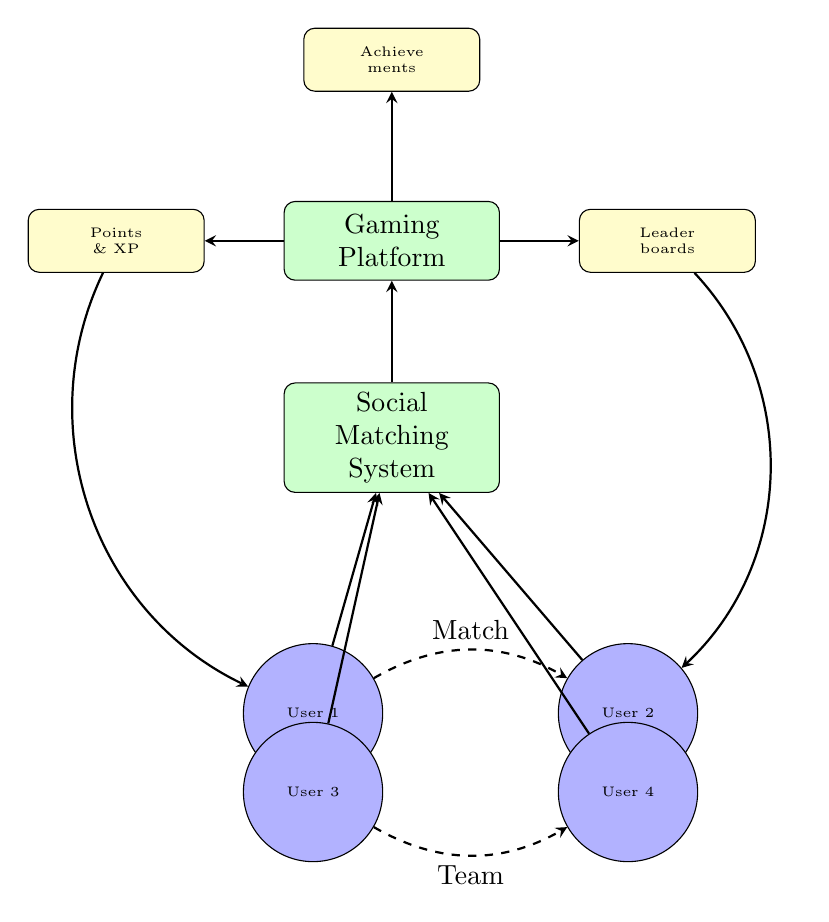
\begin{tikzpicture}[
    node distance=2cm,
    auto,
    user/.style={circle, draw, fill=blue!30, text width=1.5cm, text centered, minimum size=1.5cm, font=\tiny},
    system/.style={rectangle, draw, fill=green!20, text width=2.5cm, text centered, rounded corners, minimum height=1cm},
    game/.style={rectangle, draw, fill=yellow!20, text width=2cm, text centered, rounded corners, minimum height=0.8cm, font=\tiny},
    arrow/.style={thick,->,>=stealth},
    dashedarrow/.style={thick,->,>=stealth, dashed}
]
    % Users
    \node [user] (user1) {User 1};
    \node [user, right of=user1, xshift=2cm] (user2) {User 2};
    \node [user, below of=user1, yshift=1cm] (user3) {User 3};
    \node [user, right of=user3, xshift=2cm] (user4) {User 4};
    
    % Central system
    \node [system, above of=user1, yshift=1.5cm, xshift=1cm] (matching) {Social\\Matching\\System};
    \node [system, above of=matching, yshift=0.5cm] (gaming) {Gaming\\Platform};
    
    % Gaming elements
    \node [game, left of=gaming, xshift=-1.5cm] (points) {Points\\\& XP};
    \node [game, right of=gaming, xshift=1.5cm] (leader) {Leader\\boards};
    \node [game, above of=gaming, yshift=0.3cm] (achieve) {Achieve\\ments};
    
    % Connections
    \draw [arrow] (user1) -- (matching);
    \draw [arrow] (user2) -- (matching);
    \draw [arrow] (user3) -- (matching);
    \draw [arrow] (user4) -- (matching);
    \draw [arrow] (matching) -- (gaming);
    \draw [arrow] (gaming) -- (points);
    \draw [arrow] (gaming) -- (leader);
    \draw [arrow] (gaming) -- (achieve);
    
    % Social connections
    \draw [dashedarrow, bend left=30] (user1) to node [above, sloped] {Match} (user2);
    \draw [dashedarrow, bend right=30] (user3) to node [below, sloped] {Team} (user4);
    
    % Feedback loops
    \draw [arrow, bend right=45] (points) to (user1);
    \draw [arrow, bend left=45] (leader) to (user2);
\end{tikzpicture}
\caption{Social Gaming Integration Architecture}
\label{fig:social_gaming_architecture}
\end{figure}

\subsection{Why Gaming Works}

Gaming elements tap into fundamental human motivations:
\begin{itemize}
    \item \textbf{Achievement}: Sense of accomplishment
    \item \textbf{Competition}: Healthy rivalry and improvement
    \item \textbf{Social connection}: Shared experiences and teamwork
    \item \textbf{Progress}: Visible advancement and growth
    \item \textbf{Rewards}: Tangible and intangible benefits
    \item \textbf{Exploration}: Discovery and novelty
\end{itemize}

\subsection{Why Social Connection Matters | 为什么社交连接重要 | Warum soziale Verbindung wichtig ist}

\begin{itemize}
    \item \textbf{Reduces isolation}: Combats loneliness
    \item \textbf{Builds community}: Creates belonging
    \item \textbf{Enhances experience}: Shared moments are more memorable
    \item \textbf{Increases retention}: Social bonds bring people back
    \item \textbf{Generates word-of-mouth}: People share positive social experiences
\end{itemize}

\section{Gaming Mechanics in Hospitality | 酒店业中的游戏机制 | Spielemechaniken in der Gastronomie}

\subsection{Point and Level Systems}

\subsubsection{Experience Points (XP)}

\begin{itemize}
    \item \textbf{Visit XP}: Points for each visit
    \item \textbf{Activity XP}: Points for participating in activities
    \item \textbf{Social XP}: Points for successful social interactions
    \item \textbf{Achievement XP}: Bonus points for milestones
    \item \textbf{Referral XP}: Points for bringing friends
\end{itemize}

\subsubsection{Leveling System}

\begin{itemize}
    \item \textbf{Bronze}: New members (0-999 XP)
    \item \textbf{Silver}: Regular guests (1000-4999 XP)
    \item \textbf{Gold}: Frequent visitors (5000-14999 XP)
    \item \textbf{Platinum}: VIP members (15000+ XP)
    \item Each level unlocks new benefits and features
\end{itemize}

\subsection{Achievement System | 成就系统 | Erfolgssystem}

\subsubsection{Achievement Categories}

\begin{itemize}
    \item \textbf{Explorer}: Try different dishes, activities, rooms
    \item \textbf{Social Butterfly}: Successful matches, group activities
    \item \textbf{Competitor}: Win challenges, top leaderboards
    \item \textbf{Regular}: Consistent visits, loyalty
    \item \textbf{Ambassador}: Referrals, reviews, social sharing
    \item \textbf{Master}: Expertise in specific areas (culinary, fitness, etc.)
\end{itemize}

\subsubsection{Achievement Rewards}

\begin{itemize}
    \item Badges and recognition
    \item Exclusive access to events
    \item Special discounts
    \item Unique experiences
    \item Social status and visibility
\end{itemize}

\subsection{Leaderboards | 排行榜 | Bestenlisten}

\subsubsection{Competition Categories}

\begin{itemize}
    \item \textbf{Overall champions}: Highest total XP
    \item \textbf{Activity leaders}: Top performers in specific activities
    \item \textbf{Social stars}: Most successful matches and connections
    \item \textbf{Monthly winners}: Reset monthly for fresh competition
    \item \textbf{Team rankings}: Group-based competitions
\end{itemize}

\subsubsection{Leaderboard Features}

\begin{itemize}
    \item Real-time updates
    \item Multiple time periods (daily, weekly, monthly, all-time)
    \item Category filters
    \item Privacy options
    \item Rewards for top performers
\end{itemize}

\section{Social Matching Through Gaming | 通过游戏进行社交匹配 | Soziales Matching durch Spiele}

\subsection{Matching Algorithms | 匹配算法 | Matching-Algorithmen}

\subsubsection{Compatibility Factors}

\begin{itemize}
    \item \textbf{Interests}: Shared hobbies and activities
    \item \textbf{Activity preferences}: Similar room and experience choices
    \item \textbf{Skill levels}: Complementary or similar abilities
    \item \textbf{Social goals}: Friendship, networking, romance, collaboration
    \item \textbf{Personality traits}: Extroversion, openness, etc.
    \item \textbf{Gaming preferences}: Competitive vs. cooperative
\end{itemize}

\subsubsection{Matching Scenarios}

\begin{itemize}
    \item \textbf{Activity partners}: For fitness, cooking, gaming activities
    \item \textbf{Dining companions}: For restaurant experiences
    \item \textbf{Team formation}: For group competitions
    \item \textbf{Learning partners}: For classes and workshops
    \item \textbf{Social groups}: For events and gatherings
\end{itemize}

\subsection{Gaming as Ice Breakers | 游戏作为破冰活动 | Spiele als Eisbrecher}

\subsubsection{Conversation Starters}

\begin{itemize}
    \item \textbf{Table games}: Quick games at restaurant tables
    \item \textbf{Trivia challenges}: Food, culture, general knowledge
    \item \textbf{Cooperative puzzles}: Team problem-solving
    \item \textbf{Photo challenges}: Creative competitions
    \item \textbf{Shared quests}: Collaborative goals
\end{itemize}

\subsubsection{Team Building Games}

\begin{itemize}
    \item \textbf{Cooking challenges}: Teams prepare meals together
    \item \textbf{Escape room elements}: Problem-solving in themed rooms
    \item \textbf{Scavenger hunts}: Explore hotel and restaurant
    \item \textbf{Skill competitions}: Friendly rivalry in various activities
\end{itemize}

\section{Competitive Elements | 竞争元素 | Wettbewerbselemente}

\subsection{Individual Competitions | 个人竞赛 | Einzelwettbewerbe}

\subsubsection{Daily Challenges}

\begin{itemize}
    \item \textbf{Menu challenges}: Try specific dishes, identify ingredients
    \item \textbf{Activity challenges}: Complete specific room activities
    \item \textbf{Social challenges}: Successful matches, group participation
    \item \textbf{Skill challenges}: Improve in specific areas
\end{itemize}

\subsubsection{Weekly Tournaments}

\begin{itemize}
    \item \textbf{Culinary competitions}: Cooking challenges
    \item \textbf{Fitness tournaments}: Workout challenges
    \item \textbf{Gaming tournaments}: Video game or board game competitions
    \item \textbf{Knowledge contests}: Trivia and quiz competitions
\end{itemize}

\subsection{Team Competitions | 团队竞赛 | Teamwettbewerbe}

\subsubsection{Group Challenges}

\begin{itemize}
    \item \textbf{Team cooking}: Collaborative meal preparation
    \item \textbf{Relay activities}: Multi-room challenges
    \item \textbf{Team fitness}: Group workout competitions
    \item \textbf{Creative projects}: Art, music, or design competitions
\end{itemize}

\subsubsection{Seasonal Events}

\begin{itemize}
    \item \textbf{Quarterly championships}: Major competitive events
    \item \textbf{Special theme competitions}: Holiday or seasonal themes
    \item \textbf{Charity events}: Competitions for good causes
    \item \textbf{Community tournaments}: Open to public participation
\end{itemize}

\section{Self-Service Competition | 自助服务竞争 | Selbstbedienungswettbewerb}

\subsection{Competitive Self-Service | 竞争性自助服务 | Wettbewerbsfähige Selbstbedienung}

\subsubsection{Ordering Competitions}

\begin{itemize}
    \item \textbf{Speed challenges}: Fastest accurate order
    \item \textbf{Creativity contests}: Most innovative customizations
    \item \textbf{Accuracy competitions}: Perfect order execution
    \item \textbf{Efficiency rankings}: Optimal use of self-service features
\end{itemize}

\subsubsection{Rewards and Recognition}

\begin{itemize}
    \item Leaderboards for self-service excellence
    \item Badges for achievements
    \item Discounts and free items
    \item Recognition in app and in-restaurant
    \item Exclusive access to new features
\end{itemize}

\subsection{Social Self-Service | 社交自助服务 | Soziale Selbstbedienung}

\begin{itemize}
    \item \textbf{Group orders}: Coordinate with matched guests
    \item \textbf{Shared preferences}: Learn from successful matches
    \item \textbf{Collaborative customization}: Teams create together
    \item \textbf{Social recommendations}: See what matches are ordering
\end{itemize}

\section{Technology Platform | 技术平台 | Technologieplattform}

\subsection{Mobile Application | 移动应用 | Mobile Anwendung}

\subsubsection{Core Features}

\begin{itemize}
    \item \textbf{Profile management}: Interests, preferences, achievements
    \item \textbf{Activity booking}: Reserve rooms and experiences
    \item \textbf{Social matching}: See compatible guests, initiate connections
    \item \textbf{Gaming dashboard}: XP, levels, achievements, leaderboards
    \item \textbf{Challenge participation}: Join competitions and challenges
    \item \textbf{Self-service ordering}: Restaurant and room service
    \item \textbf{Messaging}: Communicate with matches (with consent)
    \item \textbf{Event discovery}: Find activities and social events
\end{itemize}

\subsubsection{Gaming Features}

\begin{itemize}
    \item Real-time XP tracking
    \item Achievement notifications
    \item Leaderboard updates
    \item Challenge reminders
    \item Reward redemption
    \item Progress visualization
\end{itemize}

\subsection{In-Venue Technology | 场馆内技术 | Technologie vor Ort}

\subsubsection{Interactive Displays}

\begin{itemize}
    \item \textbf{Leaderboards}: Show top performers
    \item \textbf{Activity feeds}: Real-time gaming activity
    \item \textbf{Match suggestions}: Display compatible guests
    \item \textbf{Event announcements}: Upcoming competitions
    \item \textbf{Achievement celebrations}: Recognize milestones
\end{itemize}

\subsubsection{Smart Integration}

\begin{itemize}
    \item QR codes for easy check-in and participation
    \item Wearable device integration for activity tracking
    \item Interactive tables for gaming at restaurants
    \item Room controls for functional room activities
    \item Seamless payment and rewards
\end{itemize}

\section{Privacy and Safety | 隐私与安全 | Datenschutz und Sicherheit}

\subsection{Privacy Controls | 隐私控制 | Datenschutzkontrollen}

\begin{itemize}
    \item \textbf{Profile visibility}: Control who sees your information
    \item \textbf{Matching preferences}: Set criteria for matches
    \item \textbf{Communication controls}: Who can message you
    \item \textbf{Activity sharing}: What gaming data is visible
    \item \textbf{Opt-out options}: Leave matching or gaming features
\end{itemize}

\subsection{Safety Measures | 安全措施 | Sicherheitsmaßnahmen}

\begin{itemize}
    \item \textbf{Verification}: Identity verification for matching
    \item \textbf{Reporting system}: Report inappropriate behavior
    \item \textbf{Moderation}: Staff monitoring of social interactions
    \item \textbf{Block features}: Block unwanted contacts
    \item \textbf{Emergency protocols}: Clear procedures for issues
\end{itemize}

\section{Revenue Integration | 收入整合 | Umsatzintegration}

\subsection{Gaming-Driven Revenue | 游戏驱动的收入 | Spielegetriebene Einnahmen}

\begin{itemize}
    \item \textbf{Premium memberships}: Enhanced gaming features
    \item \textbf{Competition entry fees}: For tournaments
    \item \textbf{Exclusive rewards}: Premium achievement benefits
    \item \textbf{Sponsorships}: Brand partnerships for competitions
    \item \textbf{In-app purchases}: Virtual items, boosts, features
\end{itemize}

\subsection{Social Revenue | 社交收入 | Soziale Einnahmen}

\begin{itemize}
    \item \textbf{Group bookings}: Social matching drives group visits
    \item \textbf{Event participation}: Paid social events
    \item \textbf{Premium matching}: Enhanced social features
    \item \textbf{Referral bonuses}: Rewards for bringing friends
\end{itemize}

\section{Measuring Success | 衡量成功 | Erfolg messen}

\subsection{Key Metrics | 关键指标 | Wichtige Kennzahlen}

\begin{itemize}
    \item \textbf{Engagement}: Daily active users, session length
    \item \textbf{Social connections}: Successful matches, repeat connections
    \item \textbf{Gaming participation}: Challenge completion rates
    \item \textbf{Retention}: Return visits, long-term engagement
    \item \textbf{Revenue}: Gaming and social feature revenue
    \item \textbf{Satisfaction}: Guest feedback on gaming and social features
\end{itemize}

\trilingualsection{Key Takeaways}{关键要点}{Wichtige Erkenntnisse}{}

\begin{itemize}
    \item Gaming mechanics increase engagement and retention
    \item Social matching creates value through connections
    \item Combining gaming and social elements amplifies both
    \item Competition drives participation and excitement
    \item Self-service competition adds efficiency and fun
    \item Technology enables seamless integration
    \item Privacy and safety are essential for trust
    \item Clear value proposition drives adoption
    \item Metrics help optimize the experience
    \item Balance competition with cooperation for best results
\end{itemize}

The integration of social gaming creates a unique value proposition that goes beyond traditional hospitality. For Sue and Owen, this combination represented the future of hospitality—where technology, gaming, and social connection come together to create experiences that are not just consumed, but lived and shared.
